\documentclass[a4paper,12pt,titlepage]{article}

\usepackage{listings}
\usepackage{amsmath}
\usepackage{amssymb}
\usepackage{amsthm}
\usepackage{graphicx}
\usepackage{hyperref}
\usepackage{parskip}
\usepackage{pdfpages}

\setlength{\parindent}{15pt}
\hypersetup{colorlinks=true,linkcolor=green}

\begin{document}

\title{Network Security Class \\ Lab Session 3}
\author{Stefano Zanella - 621796}
\date{July 2013}

\maketitle

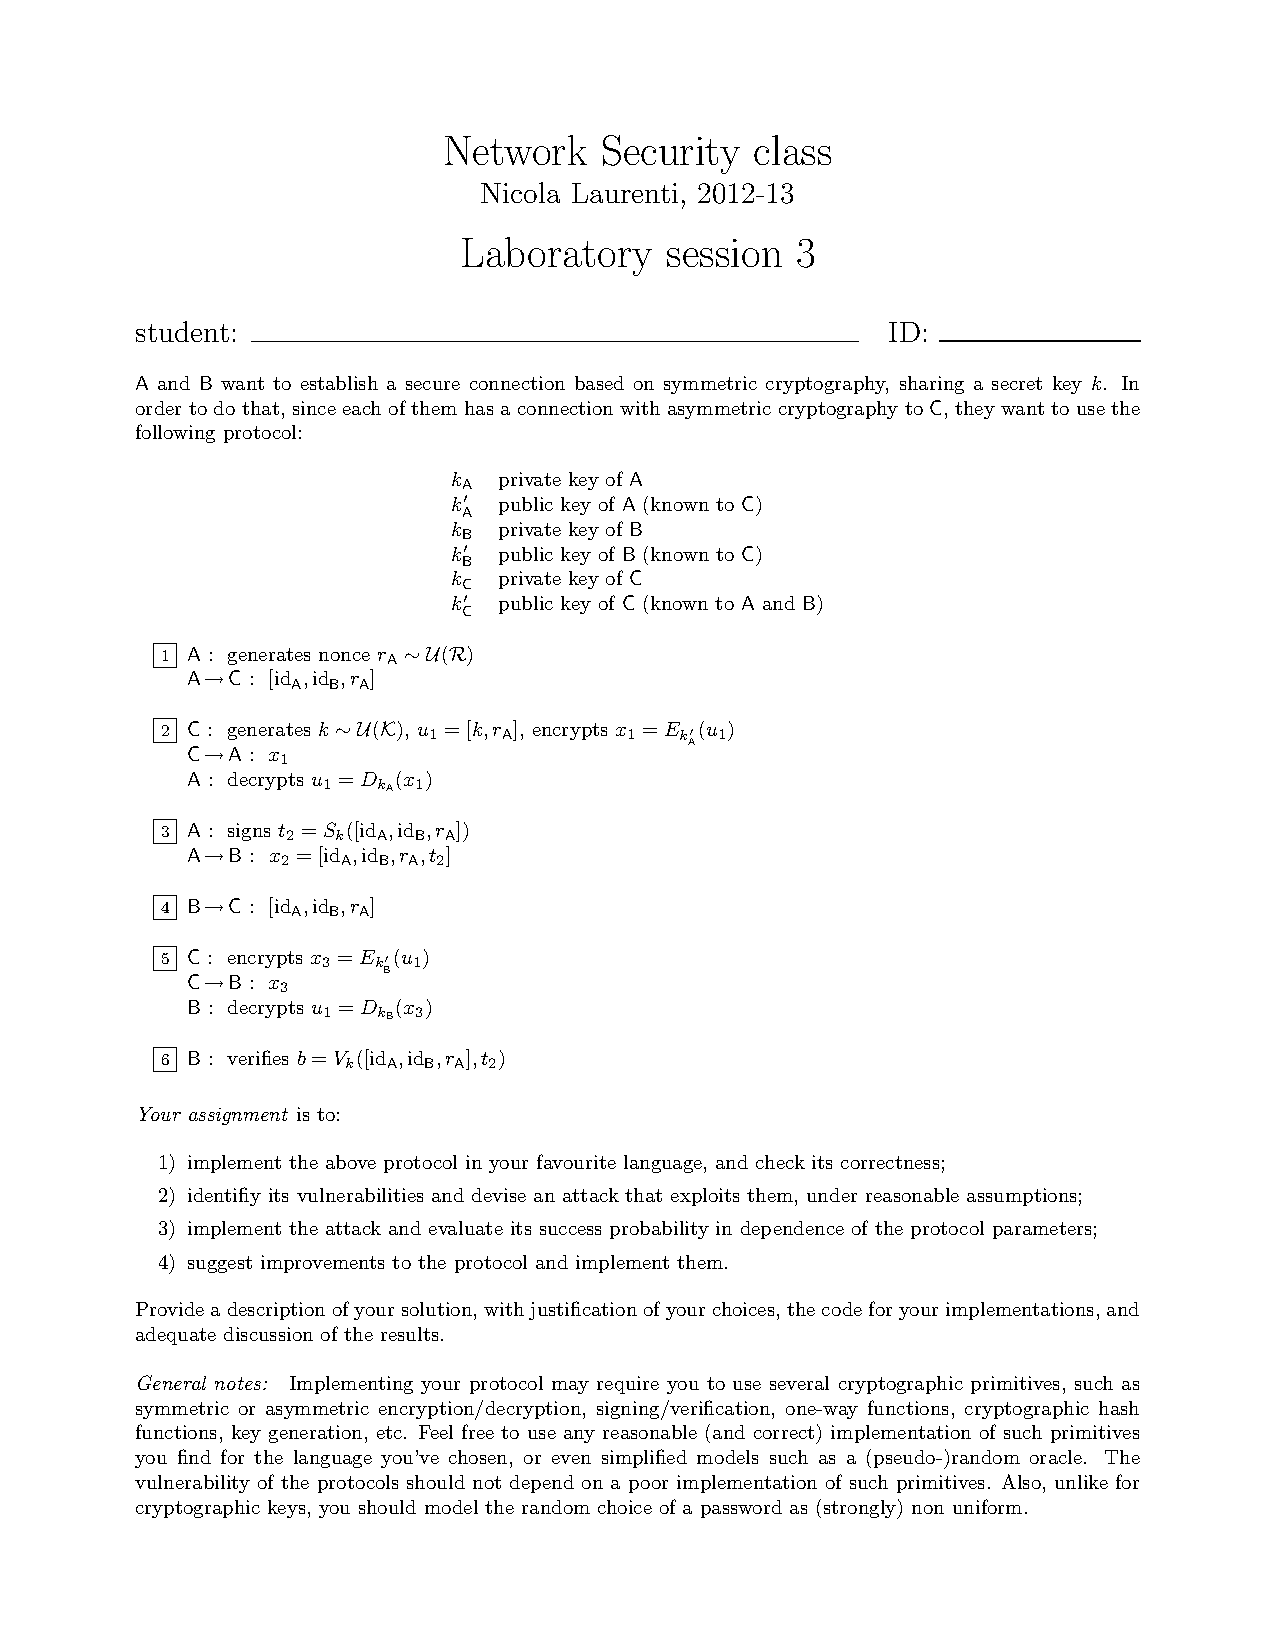
\includepdf[pages={1}]{lab_3_assignment.pdf}

\section{Implementation Details}
Here are the choices made where requested by the assignment or when no further
specification given:

\begin{itemize}
	\item The assignment has been implemented in \textbf{Ruby} (version \textbf{2.0.0-p195})
	\item To simplify the resulting codebase hosts have been modeled as classes, and
        communications over the network channel have been modeled with a \texttt{Channel}
        class that acts like a simple shared message storage. This allows to easily
        simulate message exchanging and eavesdropping.
	\item For the same reason, and to make the source code more readable, data
        concatenation has been modeled with hash maps. This in fact replaces
        specifying data chuncks' lengths in the protocol with specifying the keys at
        which data chuncks are accessible.
	\item Cryptographic primitives (ciphers, RNGs, etc.) are provided by Ruby's wrapper
        around the \textbf{OpenSSL} library and core language facilites. In detail:

    \begin{itemize}
      \item RNG is provided by the built-in \texttt{Random} class
            (\href{http://ruby-doc.org/core-2.0/Random.html}{documentation}), a PRNG based
            on a \emph{Mersenne twister}.
      \item asymmetric public key algorithm is RSA (Ruby
            \href{http://www.ruby-doc.org/stdlib-2.0/libdoc/openssl/rdoc/OpenSSL/PKey/RSA.html}{documentation}),
            with \textbf{2048 bits} key length.
      \item symmetric key cipher is \textbf{AES 256}, used when simulating communications
            between nodes.
      \item message authentication/integrity protection is provided by class \texttt{OpenSSL::HMAC}, which accepts
            an available digest algorithm as a parameter. Selected cryptographic hash
            function for message authentication is \textbf{SHA512}, provided by class
            \texttt{OpenSSL::Digest::SHA512}
            (\href{http://www.ruby-doc.org/stdlib-2.0/libdoc/openssl/rdoc/OpenSSL/Digest.html}{documentation}).
    \end{itemize}

	\item Since OpenSSL RSA works on strings, all hashes used for communication needed
  to be serialized before encryption. Ruby's built-in standard for
  serialization/deserialization is \textbf{YAML}
  (\href{http://www.ruby-doc.org/stdlib-2.0/libdoc/yaml/rdoc/YAML.html}{documentation}),
  which use is made transparent by encapsulation into class \texttt{NetSec::Node}.
\end{itemize}

\section{Protocol Implementation}
Given protocol is implemented in \texttt{NetSec::KeyExchange\#start!} method. \\
Correctness is proven at the end by printing keys hold by \textbf{A} and \textbf{B},
which are obviously the same in case the protocol works correctly.

To run the exchange, just type at the prompt, from inside the source folder:

\begin{lstlisting}[language=bash]
bin/key_agreement
\end{lstlisting}

The output should be something similar to:

\begin{lstlisting}[language=bash]
A has key: ["a2b85f3a7164c411d8ea5eb66affa741472eb59be787
                                   c3b3ea63b7816c868d39"]
B has key: ["a2b85f3a7164c411d8ea5eb66affa741472eb59be787
                                   c3b3ea63b7816c868d39"]
\end{lstlisting}

\section{Protocol Flaws and Possible Attacks}
Before describing flaws and possible attacks against them, let's just point out
a detail that is not made explicit in the assignment but seems reasonable
to assume since otherwise the protocol would be useless.

At \textbf{step 2}, after decrypting $x_1$ we'll assume that A checks that the
received $r_A$ is equal to the one generated at step 1. If this check is not
done, then there's no point in generating the nonce: at that point, even with
the improvements depicted below, it will still be possible for an attacker to
impersonate node C and send an arbitrary key to A. The same reasoning applies
symmetrically to B at \textbf{step 5}.

Also, we'll assume that at every step which involves sending identifiers (such
as step 1), the receiver verifies the id of the sender; this makes spoofing
harder and provides another level of security, easily achievable.

\subsection{C Node Spoofing}
\subsubsection*{Attack description}
While \textbf{C} makes use of asymmetric cryptography to exchange the key with
\textbf{A} and \textbf{B}, these last two does not the same when communicating with
\textbf{C}. This easily allows an attacker to spoof \textbf{C}'s identity (for example,
by DoSing it and routing requests to itself); once the attacker can
successfully impersonate \textbf{C} it has just to save the list of generated keys
and start eavesdropping from the communication channel. This way it can do
whatever it wants (from simply logging exchanged information to manipulation of
exchanged data), given no other security mechanisms are in place for a given
session (e.g. for message integrity).

\subsubsection*{Attack implementation and analysis}
To simulate spoofing of node C, a \texttt{NetSec::SpoofedC} subclass has been
introduced. Basically it acts the same way as its parent class, plus it
eavesdrop on the channel upon initialization and then saves the generated key
to decrypt eavesdropped messages.

Spoofing simulation can be run from the prompt by invoking:

\begin{lstlisting}[language=bash]
bin/spoofing_attack
\end{lstlisting}

which outputs something along the lines of:

\begin{lstlisting}[language=bash]
A has key: ["c26c3f32631b6eb395d90a63f835baccbdbc244cd400
                                   a15312bbfea15bffa93b"]
B has key: ["c26c3f32631b6eb395d90a63f835baccbdbc244cd400
                                   a15312bbfea15bffa93b"]
Spoofed C has key: ["c26c3f32631b6eb395d90a63f835baccbdbc
                           244cd400a15312bbfea15bffa93b"]
B received: My credit card number is 1234567890123456
The attacker eavesdropped: My credit card number is 
                                   1234567890123456
\end{lstlisting}

\subsubsection*{Possible improvements}
A simple solution to the problem of spoofing \textbf{C} identity would be to make
use of \textbf{C} asymmetric keys during key agreement. \\
In particular, in steps \textbf{1} and \textbf{4}, \textbf{A} and \textbf{B} could encrypt the
message $[id_A, id_B, r_A$] using \textbf{C}'s public key
$k_C'$. On the other side, \textbf{C} would then decrypt received messages
using its private key $k_C$. With this simple improvement, the only
way for an attacker to perform the same spoofing attack would be to steal
\textbf{C}'s private key, which is supposed to be an event with low probability of
success given the assumptions on which  asymmetric cryptography is based.

This solution is implemented in classes \texttt{AntispoofingA}, \texttt{AntispoofingB} and
\texttt{AntispoofingC}. The correctness of the implementation can be seen by launching
from the prompt:

\begin{lstlisting}[language=bash]
bin/antispoofing_agreement
\end{lstlisting}

To simulate the attack against this improved version, class
\texttt{SpoofedAntispoofingC} has been created. By launching

\begin{lstlisting}[language=bash]
bin/antispoofing_attack
\end{lstlisting}

it can be seen how the whole process generates an error when the malicious
\textbf{C} tries to decrypt the message from \textbf{A}'s step 1 without having the
correct private key.


\subsection{Forging Attack on A}
\subsubsection*{Attack description}
The following is not properly an attack, rather an omissis in the assignment
that has an obvious answer. However, let's see what could happen anyway.

Suppose that verification of the nonce by A at \textbf{step 2} fails. Also
suppose A wants to retry the agreement; the implementation needs to answer a
question: would A retry to send the packet and see if C answers correctly or
would she restart the agreement with a new nonce? \\
The answer is the latter, because if A is allowed to retry sending indefinitely
the same message $[id_A, r_A]$, then an attacker impersonating C, even if not
possessing $k'_C$ (but possessing $k'_A$ which we anyway assume to be
\emph{public}), can try to forge $[k, r_A]$ until it's accepted by A.
In the context of the simulation failures and retries are not considered to
keep complexity low, but this issue can easily be addressed once we're able to
identify the failure (more on this later).

\subsection{KPA Attack}
\subsubsection*{Attack description}
In given implementation, there is room for a KPA attack on $k'_C$: if we
consider C node spoofing solved (see above), then an attacker can
gain pairs of known plain and ciphertext by gathering the message sent at step
1 from A to C, and the signed message sent from A to B at step 3. By discarding
the signature, the attacker has access to a potentially unlimited amount of
pairs (since keypairs aren't changed often) that can be used for an offline
attack against C's private key.

\subsubsection*{Attack implementation and analysis}

\subsubsection*{Possible improvements}
A solution of this issue, which also brings half of another desirable feature,
is to:
\begin{itemize}
  \item modify step 2 so that C also sends $k'_B$ to A
  \item modify step 3 so that A sends $\hat{x_2} = E_{k'_B}(x_2)$ instead of $x_2$
  \item modify step 4 so that B first decrypts $x_2 = D_{k_B}(\hat{x_2})$, then
  sends $x_2$ to C
\end{itemize}
The advantage of this approach is that it allows A to authenticate B, since
only B is supposed to be able to decrypt $\hat{x_2}$.

\section{Furhter improvements}
We've stated that, in the attempt to avoid the possibility of a KPA, we've
introduced authentication of B to A. While not strictly needed, we can think of
also performing the other side of the authentication by symmetrically adapting
the protocol on the B side. That is, we could let C send to B $k'_A$ at step 5;
then, after correctly verifying signature from A, B could simply send a
challenge $E_{k'_A}(r_B),\; r_B \sim \mathcal{U}(\mathcal{R})$. At this point,
A would just decrypt $r_B$ and send back $E_k(r_B - 1)$ (so to check that $k$
works as expected). This way the protocol would also implement mutual public
key authentication (again, not strictly needed given the purpose of the
protocol).

\section{Open Question}
An open question remains, which doesn't count too much for the purposes of this
simulation, but gains relevance as soon as we try to adapt protocol to real
world, which is: how to handle and notify failures in key agreement in a secure
way?

That is, in the simulation when a failure happens due to a failed attack, it's
easy to stop the agreement by just raising an exception. This works well
because we're running inside a single program, but can't be a solution when
nodes are physically distinct machines. As long as the failure happens at A
the problem doesn't arise: since it's A to have
initiated the agreement, it can just retry as explained or stop trying. \\
But, suppose a failure happens at C in the middle of the exchange with A: what
should C do? Probably the safest thing to do is to just not send any answer,
letting A wait and eventually decide to drop the tentative by timeout. But, if
A is a legitimate sender, then such behaviour would result in a loss of
performance, which may or may not be mitigated/accepted with timeout tuning. On
the other side, letting A know explicitly about the failure, would give
information to an eventual attacker that could modify his success probability
to his advantage. \\
The same question applies when the failure happens at B, which also arise the
problem of how to let A know of the failure, again without giving a possible
attacker any specific information that could be used to his advantage.
\end{document}
